\chapter{Introduction}

D. L. Parnas published a paper titled \textit{On the Criteria To Be Used in Decomposing Systems into Modules}\cite{parnaDecomposing} in 1972. Since then, decomposition of software systems has become an important area in the field of software engineering. As systems grew more complex, software engineers started to distribute modules over in computer networks and hence called them services. Architectural styles like Software Oriented Architecture (SOA) have been introduced to tackle the many challenges such distributed systems create. 

Nevertheless, even with microservices, the latest incarnation of service orientation, decomposition is more described as an art than a structured discipline. C. Richardson writes in his popular introduction to microservices on \gls{infoq}:

\begin{quote}
	\textit{Deciding how to partition a system into a set of services is very much an art but there are number of strategies that can help. One approach is to partition services by verb or use case.}\cite{richardson2014microservices}
\end{quote}

As we acknowledge the suitability of the described strategies, we do believe that there is a more structured way to service decomposition. This leads us to our first hypothesis:

\begin{quote}
	\textit{The driving factors for service cuts in a software system can be compiled into a comprehensive criteria catalog.}
\end{quote}

To validate this first hypothesis, we created a catalog of coupling criteria as a product of the thesis. Taking this structured approach to service decomposition a step further, we formulated a second hypothesis:

\begin{quote}
	\textit{The data of the criteria catalog can be embodied in a tool to optimize loose coupling between and high cohesion within services in a structured and automated way.}
\end{quote}

To validate this second hypothesis, we developed a prototype based on the criteria catalog. This prototype, hence called the \enquote{Service Cutter}, analyses a system's specification and suggests candidate service cuts in order to optimize loose coupling between services and high cohesion within services. A system's specification contains a domain model, use cases and further artifacts as illustrated in Figure \ref{fig:serviceCutterIO}.

\begin{figure}[H]
	\begin{center}
		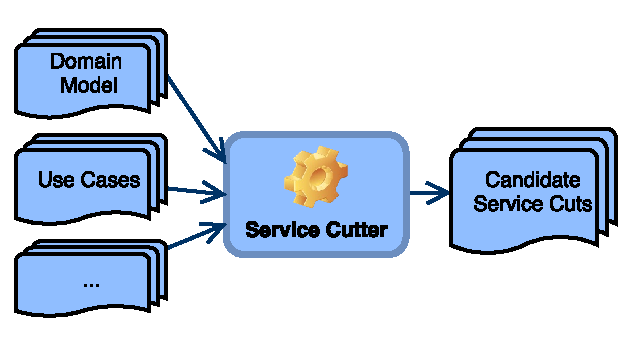
\includegraphics[scale=1.1]{diagrams/systemContextDiagram.pdf}
	\end{center}
	\caption{Input and Output of Service Cutter}
	\label{fig:serviceCutterIO}
\end{figure}



The Service Cutter's goal is to assist and advise a software architect or developer in his design decisions regarding service decomposition. The architect needs to assess the candidate service cuts and compare them with his expectations. The Service Cutter's mission is accomplished, if the architect's expectations are verified or unexpected but reasonable candidate cuts challenge his preoccupations. 

\section{Project Definition}

The original project definition, signed at the beginning of project, is documented in Appendix \ref{appendix:projectDefinition}.

\section{Context and Influences}

The ideas and concepts in this thesis are influenced by the work of many others. We reused and embodied existing concepts to our structured way of service decomposition. This section describes the context and influences of the thesis.

\subsection{Service Oriented Architecture}

It was during a course titled \textit{Advanced Distributed Systems Design using SOA \& DDD} by Udi Dahan where our initial idea to assist service decomposition with an automated approach emerged. Dahan is the founder of NServiceBus\cite{nservicebus}, the most popular service bus for \gls{dotnet} and a well known \gls{SOA} and \gls{DDD} expert. The approach to tackle service decomposition from the 4+1 View Model\cite{fourPlusOne} is inspired by him. Approaching decomposition on the basis of data fields, or the later in the document introduced nanoentites, is motivated by his course.

Further \gls{SOA} influences are provided by our supervisor Dr. Prof. O. Zimmermann throughout the project and during his course \textit{Application Architecture} at \gls{HSR}.

\subsection{Microservices}

In recent years, microservices substituted \gls{SOA} as the trending architectural style, but can be seen as a new incarnation of the service oriented approach. Valuable concepts like service definitions or decomposition criteria are inspired by leading evangelists in this area such as Martin Fowler, Sam Newman, and Chris Richardson. 

\subsection{Domain-Driven Design}

Nevertheless, decomposition is not solely a problem in distributed systems. Eric Evans introduced in his book \textit{Domain-Driven Design: Tackling Complexity in the Heart of Software}\cite{evans2003domain} a collection of patterns to handle decomposition complexity. Especially the concepts of \textit{Bounded Context}, \textit{Entity}, \textit{Published Language} were integrated in our approach.

\section{Scope}

This section describes the scope and boundaries of this thesis. 

Throughout the document, a \textit{system} refers to a software application which needs to be built and therefore decomposed. 

A \textit{service} can be seen as a module providing a remote \gls{API} to communicate with other services. The term is explained in more detail in Chapter \ref{cha:analysis}

\textit{Service decomposition} refers to splitting a system's functionality and data into services. While we focus on service decomposition, most of the concepts are also true for non-distributed systems where a software internally is decomposed into modules. 

Before a system can be decomposed, its functional and non-functional requirement need be be analyzed and specified in a domain model, use cases, and other artifacts. Based on these specifications the system can be decomposed into services. These are later implemented and connected using intra service communication. Figure \ref{fig:context} illustrates this process.

\begin{figure}[H]
	\begin{center}
		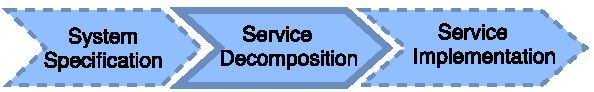
\includegraphics[scale=1.4]{diagrams/context.pdf}
	\end{center}
	\caption{The thesis in the context of system development}
	\label{fig:context}
\end{figure}

Our thesis focuses solely on service decomposition. Consequently the following areas are not in scope:

\begin{itemize}
	\item Requirements engineering and system specification need to be done before a system can be analyzed with the Service Cutter.
	\item Intra service communication is not in scope of this thesis. S. Newman documents in his book \textit{Building Microservices}\cite{newman2015building} multiple popular ways for intra service communication like \gls{RPC}, RESTful HTTP services or asynchronous event-based collaboration. Decomposition only defines \textit{what} is communicated but now \textit{how}. 
	\item Composing multiple services into workflows or business processes using notations like \gls{BPMN} is not in scope.
	\item Service decomposition tries to minimize coupling between services. Tactics like caches or \gls{CQRS}, which try to lower the consequences of coupling introduced by decomposition, are not analyzed. 
\end{itemize}

\bigskip

After introducing our hypothesis's and goals, the next Chapter analyzes the definition of a service and service decomposition principles in more detail. 

%TODO AppArch 3 Ebenen von Services,  Drei definitionen von SOMA/Services, User / Architect / Developer